\usetikzlibrary{positioning}
\chapter{Approaches for Neural PDE Simulators}
\label{chap:approaches}

% ----------------------------------------------------------- SAMUEL MODEL -------------------------------------------------------------------------------
\section{Approach 1: Samuel's Model}
\subsection{Model Architecture}
\subsection{}


% ----------------------------------------------------------- ALEX MODEL -------------------------------------------------------------------------------
\section{Approach 2: Causal Temporal Convolutional Attention Network}
\subsection{Model Architecture}
The Causal Temporal Convolutional Attention Network (TCAN) is a feed-forward autoregressive model that predicts next state of a PDE given a sliding window of past states. At each time step, the model receives a history window $u_{\text{history}}$ of shape $(B, W, P)$---where $B$ is the batch size, $W$ is the history length (e.g., 20), and $P$ is the number of spatial grid points---and outputs the next field $u_{t+1}$ of shape $(B, 1, P)$. The model operates as a one-step neural PDE surrogate, repeatedly applied in an autoregressive rollout to generate full trajectories.\\\\
The architecture consists of three main components:\\
1. A temporal attention encoder that aggregates information across the history window.\\
2. A convolutional decoder that produces a bounded correction.\\
3. A residual update that adds the correction to the last frame.\\\\
The full data flow for a single prediction step is illustrated in Figure~\ref{fig:tcn-flow}.

\begin{figure}[htbp]
\centering
\resizebox{0.95\textwidth}{!}{%
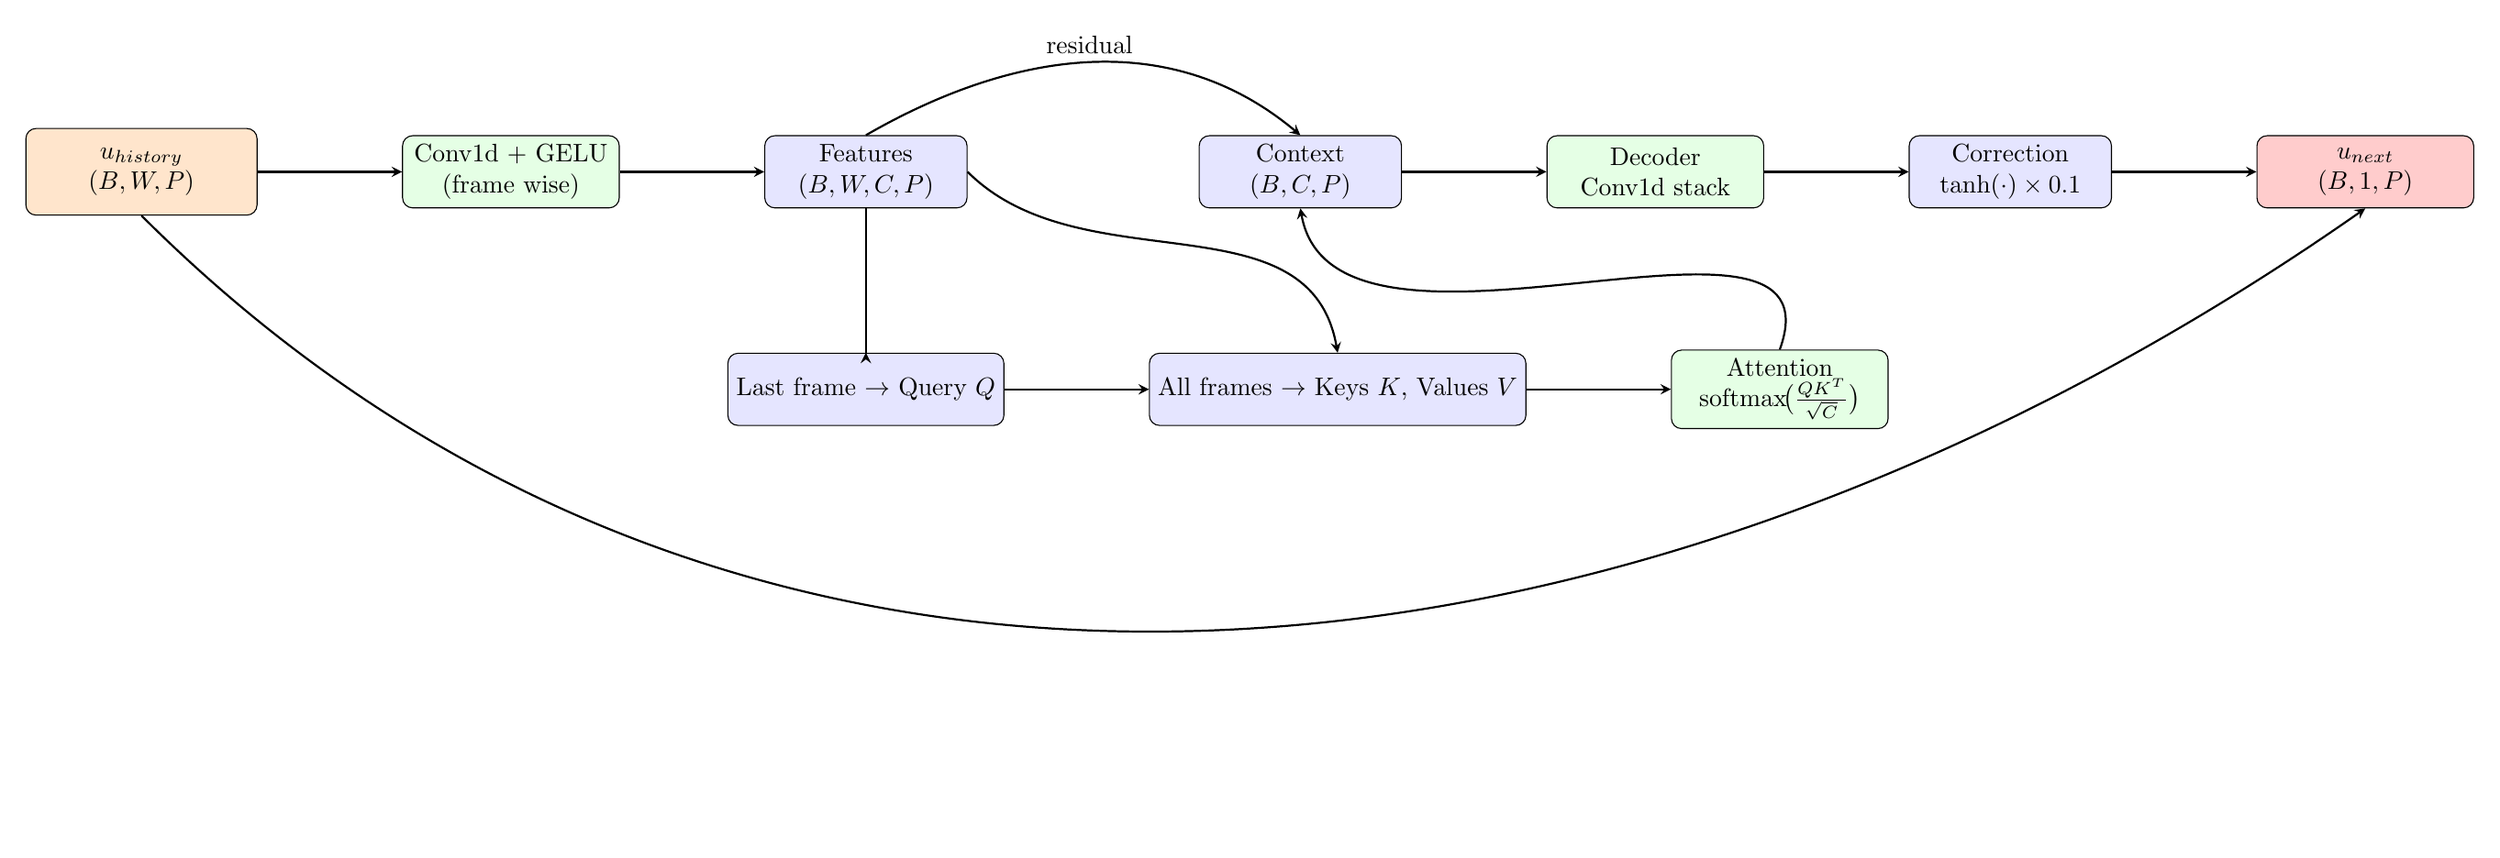
\begin{tikzpicture}[
    box/.style={rectangle, draw, rounded corners, minimum width=2.8cm, minimum height=1cm, align=center, fill=blue!10},
    op/.style={rectangle, draw, rounded corners, minimum width=3cm, minimum height=1cm, align=center, fill=green!10},
    arrow/.style={->, thick, >=stealth},
    input/.style={rectangle, draw, rounded corners, minimum width=3.2cm, minimum height=1.2cm, align=center, fill=orange!20},
    output/.style={rectangle, draw, rounded corners, minimum width=3cm, minimum height=1cm, align=center, fill=red!20},
    node distance=2.0cm
]

% Fila superior: flujo principal
\node[input] (input) {$u_{\text{history}}$\\$(B, W, P)$};
\node[op, right=of input] (embed) {Conv1d + GELU\\(frame wise)};
\node[box, right=of embed] (features) {Features\\$(B, W, C, P)$};
\node[box, right=3.2cm of features] (context) {Context\\$(B, C, P)$};
\node[op, right=of context] (decoder) {Decoder\\Conv1d stack};
\node[box, right=of decoder] (corr) {Correction\\$\tanh(\cdot)\times 0.1$};
\node[output, right=of corr] (output) {$u_{\text{next}}$\\$(B, 1, P)$};

% Fila inferior: atención temporal
\node[box, below=2.0cm of features] (query) {Last frame $\rightarrow$ Query $Q$};
\node[box, right=of query] (kv) {All frames $\rightarrow$ Keys $K$, Values $V$};
\node[op, right=of kv] (attn) {Attention\\$\mathrm{softmax}\!\big(\frac{QK^{T}}{\sqrt{C}}\big)$};

% Flechas flujo principal (superior)
\draw[arrow] (input) -- (embed);
\draw[arrow] (embed) -- (features);
\draw[arrow] (context) -- (decoder);
\draw[arrow] (decoder) -- (corr);
\draw[arrow] (corr) -- (output);

% Flecha a Query: igual que antes
\draw[arrow] (features.south) |- (query.north);

% Flecha a Keys/Values: menos baja, gira antes a la derecha
\draw[arrow] (features.east) to[out=-45,in=100] (kv.north);

% Flechas dentro de la rama de atención
\draw[arrow] (query) -- (kv);
\draw[arrow] (kv) -- (attn);

% De atención a contexto: giro bajo
\draw[arrow] (attn.north) to[out=70,in=-80] (context.south);

% Residual de features a context (por arriba)
\draw[arrow] (features.north) to[out=30,in=140] node[above]{residual} (context.north);

% Residual de u_history a u_next (sin texto, menos alto)
\draw[arrow] (input.south) to[out=-45,in=-145] (output.south);

\end{tikzpicture}%
}
\caption{Data flow through the Causal Temporal Attention Network during one prediction step.}
\label{fig:tcn-flow}
\end{figure}


\subsection{Temporal Attention Encoder}

The \texttt{CausalTemporalAttention} module processes the history window through the following steps:

\begin{enumerate}
    \item \textbf{Frame-wise embedding}: Reshape $u_{\text{history}}$ to $(B \cdot W, 1, P)$ and apply a 1D convolution with kernel size 3 followed by GELU activation, producing features of shape $(B \cdot W, C, P)$ where $C=32$ is the embedding dimension.
    
    \item \textbf{Temporal restructuring}: Reshape features back to $(B, W, C, P)$ to expose the temporal dimension.
    
    \item \textbf{Query computation}: Extract features of the last frame $\text{features}[:, -1, :, :] \in \mathbb{R}^{B \times C \times P}$ and apply a $1 \times 1$ convolution to obtain queries $Q \in \mathbb{R}^{B \times C \times P}$.
    
    \item \textbf{Key and value projection}: Apply $1 \times 1$ convolutions to all $W$ frames (flattened to $(B \cdot W, C, P)$ then reshaped) to obtain keys $K$ and values $V$, both of shape $(B, W, C, P)$.
    
    \item \textbf{Causal attention scores}: Compute scaled dot-product attention over the temporal dimension:
    \[
    \text{scores}_{b,w,p} = \frac{\langle Q_b, K_{b,w} \rangle}{\sqrt{C}}, \quad \alpha_{b,w,p} = \text{softmax}_w(\text{scores}_{b,w,p})
    \]
    
    \item \textbf{Context aggregation}: Compute the attended context:
    \[
    \text{context}_b = \sum_{w=1}^W \alpha_{b,w} \cdot V_{b,w} \in \mathbb{R}^{B \times C \times P}
    \]
    
    \item \textbf{Residual projection}: Apply a $1 \times 1$ convolution to the context, add the residual connection to the last frame features, and normalize with GroupNorm.
\end{enumerate}

This mechanism allows the last frame to dynamically query relevant past frames at each spatial location, producing spatially-aware temporal context features.

\subsection{Decoder and Residual Correction}

The \texttt{ImprovedBurgersNet} decoder processes the attention output $\text{context} \in \mathbb{R}^{B \times C \times P}$ as follows:

\begin{enumerate}
    \item \textbf{Convolutional decoder stack}:
    \begin{itemize}
        \item Conv1d: $C \to 32$ channels, kernel size 5, BatchNorm1d, GELU.
        \item Conv1d: $32 \to 1$ channel, kernel size 5, producing $\text{raw\_correction} \in \mathbb{R}^{B \times 1 \times P}$.
    \end{itemize}
    The final layer is zero-initialized to ensure near-zero corrections during early training.
    
    \item \textbf{Bounded correction}: Apply hyperbolic tangent clipping scaled by $\text{corr\_clip}=0.1$:
    \[
    \Delta u = \tanh(\text{raw\_correction}) \cdot 0.1
    \]
    
    \item \textbf{Residual update}: Add the correction to the last input frame:
    \[
    u_{\text{next}} = u_{\text{history}}[:, -1:, :] + \Delta u
    \]
\end{enumerate}

This design enforces incremental updates, preventing instability during long autoregressive rollouts.

\subsection{Autoregressive Training Procedure}

Training employs curriculum learning with multi-step rollouts:

\begin{enumerate}
    \item Initialize $\text{current\_window} = u_{\text{gt}}[:, :W, :]$ from ground truth trajectories.
    
    \item For each rollout step $k \in \{0, \dots, D-1\}$ where $D$ is the rollout depth (curriculum: 8$\to$16$\to$64):
    \begin{itemize}
        \item Predict $\hat{u}_{W+k} = \text{TCAN}(\text{current\_window})$.
        \item Compute composite loss:
        \[
        \mathcal{L} = \text{MSE}(\hat{u}, u_{\text{gt}}) + 0.1 \cdot \|\nabla_x \hat{u} - \nabla_x u_{\text{gt}}\|_2^2 + 0.05 \cdot \mathbb{E}[\max(0, E(\hat{u}) - E(u_t))]
        \]
        where $E(u) = \frac{1}{2} \int u^2 \, dx$ enforces energy dissipation.
        \item Update window: $\text{current\_window} \gets [\text{current\_window}[:, 1:, :], \hat{u}]$ (with occasional teacher forcing).
    \end{itemize}
    
    \item Average loss over rollout, backpropagate through unrolled computation graph, apply gradient clipping, and optimize with AdamW + cosine annealing.
\end{enumerate}

\subsection{Evaluation Metrics}

Full-trajectory predictions are evaluated using:
\begin{itemize}
    \item Standard: MSE, relative $L^2$, PSNR, SSIM, temporal correlation.
    \item Physics-informed: mass conservation error, energy monotonicity fraction, mean PDE residual, spectral error, max gradient error.
\end{itemize}

This comprehensive evaluation ensures both accuracy and physical fidelity across long rollouts.
